\documentclass[tikz]{standalone}
\usetikzlibrary{intersections}
\begin{document}
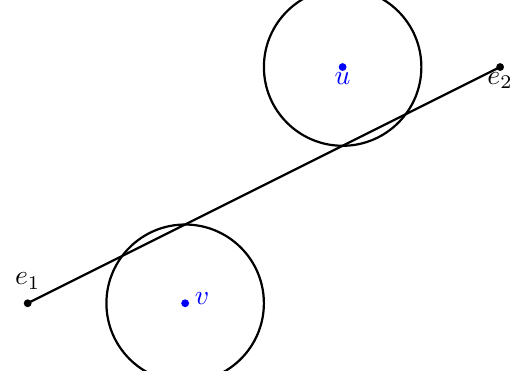
\begin{tikzpicture}
  \useasboundingbox (0,3.5) rectangle (6,-0.5);

  \coordinate (e1) at (0, 0);
  \coordinate (e2) at (6, 3);
  \coordinate (v)  at (2, 0);
  \coordinate (u)  at (4, 3);

  \draw[thick] (e1) -- (e2);

  \draw[thick] (u) circle (1);
  \draw[thick] (v) circle (1);

  \path[name path=line] (e1) -- (e2);
  \path[name path=circleu] (u) circle (1);
  \path[name path=circlev] (v) circle (1);
  \path[name intersections={of=line and circleu, by={tu0,tu1}}];
  \path[name intersections={of=line and circlev, by={tv1,tv0}}];

  \node[circle,fill,color=black,inner sep=1pt,label={[text=black, above]:\(e_1\)}] at (e1) [] {}; 
  \node[circle,fill,color=black,inner sep=1pt,label={[text=black, below]:\(e_2\)}] at (e2) [] {}; 

  \node[circle,fill,color=blue,inner sep=1pt,label={[text=blue, below]:\(u\)}] at (u) [] {}; 
  \node[circle,fill,color=blue,inner sep=1pt,label={[text=blue, right]:\(v\)}] at (v) [] {}; 
\end{tikzpicture}
\end{document}
